\chapter{XSL, XPath, and XSLT}\label{a1}
\markboth{Appendix~\ref{a1}. XSL, XPath, and XSLT}{}

\section{Extensible Stylesheet Language (XSL)}\label{XSL}
\markright{~\ref{XSL} Extensible Stylesheet Language (XSL)}

\begin{figure}[h]
\begin{center}
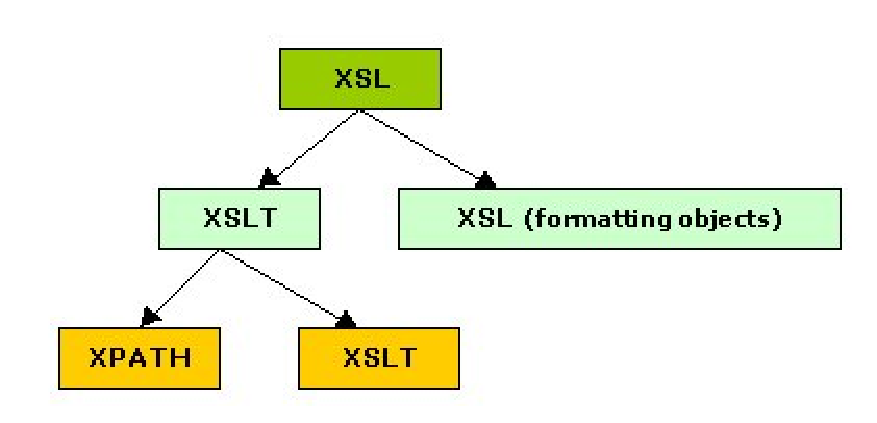
\psfig{file=Figures/esquema.eps,scale=.75}
\end{center}
\caption{Schema of the relationship between XSL, XPath, and XSLT.}
\label{FigureA1}
\end{figure}

The Extensible Stylesheet Language (XSL) \cite{W3C2006} is a language developed by the W3C based on XML that is used to specify how the information in an XML document is transformed to create a new document. This new document can be another XML document, an HTML we want to display in a browser, \ldots\ XSL language was formerly divided into two parts: (i) a transformation language specifying how the transformation between documents is done, and (ii) a formatting language specifying how the resulting XML documents will be.

During the development of the XSL standard the transformation language was split into a different specification called Extensible Stylesheet Language Transformations (XSLT). Moreover, the part of the XSLT language responsible for accessing and navigating the nodes of the XML document was also split into another language. This language was called XML Path Language (XPath) and is intended to be used together with XSLT.

In Figure \ref{FigureA1} we can see a schema showing the relationship between these three specification languages.

\section{XML Path Language (XPath)}\label{XPath}
\markright{~\ref{XPath} XML Path Language (XPath)}

XML Path Language (XPath) \cite{W3C1999} is a language used to find information inside an XML document. The language allows us to navigate across the different elements and attributes composing the document.

XPath uses \textbf{path expressions} to do the nodes selection inside the XML document. These expressions are very similar to the paths used by file systems in operating systems like Windows or Linux.

XPath also provides more than 100 \textbf{functions} offering capabilities such as manipulation of strings, manipulation of numerical values, data comparisons, \ldots

In XPath we can distinguish seven different types of node: root nodes, element nodes, text nodes, attribute nodes, namespace nodes, processing instruction nodes and comment nodes. An XML document is treated as a tree of these nodes, where we have the following relationships between the nodes:

\begin{itemize}

\item \textbf{Parent}: Each element in the document has a parent except the root node.

\item \textbf{Children}: Each element can have zero, one or more children.

\item \textbf{Siblings}: Elements with the same parent are considered siblings.

\item \textbf{Ancestor}: We consider ancestors of an element its parent, its parent's parent, \ldots

\item \textbf{Descendant}: We consider descendants of an element its children, its children's children, \ldots

\end{itemize}

The selection of nodes in XPath is done by following a path. Some of the most common path expressions are the following, where several of them can be combined by means of the operator \textbf{$|$}:

\begin{itemize}

\item \textbf{nodename}: It selects all the children with name \textit{nodename}.

\item \textbf{/}: It selects from the root node.

\item \textbf{//}: It selects the nodes in the document satisfying the selection condition given next, without taking into account the place in the hierarchy where they are.

\item \textbf{.}: It selects the current node.

\item \textbf{..}: It selects the parent of the current node.

\item \textbf{@}: It selects attributes of the node.

\end{itemize}

Predicates are used in XPath to find a node having an specific name or containing an specific value. These predicates are always written inside square brackets (\textit{[]}) and some of the most common are the following, where the symbol \textbf{*} can be used as a wildcard:

\begin{itemize}

\item \textbf{nodename[1]}: It selects the first child of the current node with name \textit{nodename}.

\item \textbf{nodename[last()]}: It selects the last child of the current node with name \textit{nodename}.

\item \textbf{nodename[position $<$ 3]}: It selects the first two children of the current node with name \textit{nodename}.

\item \textbf{nodename[@lang]}: It selects the children of the current node with name \textit{nodename} and having an attribute \textit{lang}.

\item \textbf{nodename[@lang=``es'']}: It selects the children of the current node with name \textit{nodename} and having an attribute \textit{lang} with value \textit{``es''}.

\item \textbf{nodename[price $>$ 20]}: It selects the children of the current node with name \textit{nodename} and having a child element named \textit{price} with a value over \textit{20}.

\end{itemize}

Axes are used in XPath to define a set of nodes relative to the current node. The axes defined in the language are the following:

\begin{itemize}

\item \textbf{ancestor}: It selects all the ancestor nodes of the current node.

\item \textbf{ancestor-or-self}: It selects all the ancestor nodes of the current node and the current node itself.

\item \textbf{attribute}: It selects all the attributes of the current node.

\item \textbf{child}: It selects all the children of the current node.

\item \textbf{descendant}: It selects all the descendants of the current node.

\item \textbf{descendant-or-self}: It selects all the descendants of the current node and the current node itself.

\item \textbf{following}: It selects all the elements in the document after the closing label of the current node.

\item \textbf{following-sibling}: It selects all the subsequent siblings of the current node.

\item \textbf{namespace}: It selects all the namespace nodes inside the current node.

\item \textbf{parent}: It selects the parent of the current node.

\item \textbf{preceding}: It selects all the elements in the document before the opening label of the current node.

\item \textbf{preceding-sibling}: It selects all the previous siblings of the current node.

\item \textbf{self}: It selects the current node.

\end{itemize}

There are also a set of operators that can be used in XPath expressions. They are the following:

\begin{itemize}

\item \textbf{$|$}: It is used to combine two sets of nodes.

\item \textbf{+}: Addition.

\item \textbf{-}: subtraction;.

\item \textbf{*}: Multiplication.

\item \textbf{div}: Division.

\item \textbf{=}: Equality.

\item \textbf{!=}: Inequality.

\item \textbf{$<$}: Less than.

\item \textbf{$<$=}: Less or equal than.

\item \textbf{$>$}: Greater than.

\item \textbf{$>$=}: Greater or equal than.

\item \textbf{or}: Logic operator ``or''.

\item \textbf{and}: Logic operator ``and''.

\item \textbf{mod}: Modulus operator.

\end{itemize}

Finally, XPath also provides a library of functions for multiple purposes: error functions, numeric functions, string manipulation functions, date functions,\ldots

\section{Extensible Stylesheet Language Transformations (XSLT)}\label{XSLT}
\markright{~\ref{XSLT} Extensible Stylesheet Language Transformations (XSLT)}

Extensible Stylesheet Language Transformations (XSLT) \cite{W3C1999-2} is the most important part of XSL. By using XSLT we can add or delete elements and attributes in the generated output document. It also allows us to order elements, make queries and make decisions about which elements are included and which elements are not included in the output document

In the process of transformation, XSLT uses XPath to define parts of the input document that must correspond with one or several templates. If one of these parts is found in the input document, XSLT does the transformation of it into the output document.

The root element of an XSLT document is always $<$xsl:stylesheet$>$ or $<$xsl:transform$>$.

The element $<$xsl:template$>$ is used to build templates. The attribute \textit{match} is used to match a template with an XML element. To define a template corresponding to the full XML document, this attribute must have the value \textbf{/}.

The element $<$xsl:value-of$>$ is used to extract a value from the input XML and adding it to the output XML, using the attribute \textit{select} for this purpose.

The element $<$xsl:sort$>$ is used to order the output by including this element inside element $<$xsl:for-each$>$ and 
using the attribute \textit{select} to specify the ordination criteria.

The element $<$xsl:if$>$ is used to evaluate a condition and its internal code is only executed if this condition is fulfilled, otherwise its code would have no effect. The attribute \textit{test} is used to specify the condition.

The element $<$xsl:choose$>$ is used together with the elements $<$xsl:when$>$ and $<$xsl:otherwise$>$ to evaluate multiple conditions.

The element $<$xsl:apply-templates$>$ applies a template over the current node or over the children of the current node. If the attribute \textit{select} is included only the children corresponding to the attribute value will be processed. In this way, the attribute can be used to determine the order in which children are processed.

There are still more elements that can be used in XSLT: the element \textit{text} to directly write any text in the output document, the element \textit{element} to create the specified node in the output document, the element \textit{call-template} to call templates by means of their name, \ldots